\documentclass[11pt,a4paper]{article}

\usepackage[utf8]{inputenc}
\usepackage[T1]{fontenc}
\usepackage[french]{babel}
\usepackage{geometry}
\usepackage{graphicx}
\usepackage{booktabs}
\usepackage{array}
\usepackage{float}
\usepackage{caption}
\usepackage{hyperref}

\geometry{margin=2.5cm}
\setlength{\parskip}{0.45em}
\setlength{\parindent}{0pt}

\title{Rapport de description des donn\'ees\newline Feux en for\^et bor\'eale}
\author{Projet Foret Boreale}
\date{\today}

\begin{document}
\maketitle

\section{Objectif et p\'erim\`etre}
Ce rapport d\'ecrit les donn\'ees exploit\'ees dans le notebook \texttt{Analyse\_exploratoire\_donnees.ipynb} et reprend les figures export\'ees dans \texttt{figures\_feu/}. L'objectif est de documenter clairement la structure des fichiers, les variables disponibles et les grands motifs temporels observ\'es avant toute mod\'elisation.

Les r\'ef\'erences utiles pour le contexte m\'ethodologique sont le notebook d'exploration des donn\'ees, le document technique sur l'architecture des mod\`eles s\'equentiels et la pr\'esentation de synth\`ese du projet~\cite{nb_explo,doc_modeles,pres_feu}.

\section{Jeux de donn\'ees retenus}
Le tableau~\ref{tab:sources} r\'esume les fichiers principaux utilis\'es dans l'analyse du feu.

\begin{table}[H]
\centering
\begin{tabular}{p{4.5cm} p{2.2cm} p{2.2cm} p{5.5cm}}
\toprule
\textbf{Fichier} & \textbf{Taille} & \textbf{Format} & \textbf{R\^ole dans l'analyse} \\
\midrule
\texttt{FFBootCISap.csv} & 13\,063 lignes & large & Fr\'equence r\'egionale du feu (FF) \\
\texttt{BBBootCISap.csv} & 13\,063 lignes & large & Biomasse br\^ul\'ee r\'egionale (BB) \\
\texttt{FSBootCISap.csv} & 13\,063 lignes & large & Indice de taille / s\'ev\'erit\'e (FS) \\
\texttt{Lake\_fire\_frequency\_24nov2023.csv} & 83 lignes $\times$ 6 colonnes & large & Occurrences de feu par lac \\
\bottomrule
\end{tabular}
\caption{Fichiers principaux mobilis\'es dans le rapport.}
\label{tab:sources}
\end{table}

\subsection*{Structure des proxys r\'egionaux}
Les fichiers \texttt{FFBootCISap.csv}, \texttt{BBBootCISap.csv} et \texttt{FSBootCISap.csv} partagent la m\^eme structure: 
\texttt{Age}, \texttt{Mean}, \texttt{CI}, \texttt{Infe} et \texttt{Supe}. La colonne \texttt{Age} couvre ici l'intervalle \(-62\) \`a 13\,000 ans, tandis que \texttt{Mean} encode le signal central et que \texttt{Infe}/\texttt{Supe} fournissent un intervalle de confiance \`a 90\%.

Les ordres de grandeur observ\'es sont diff\'erents selon le proxy:
\begin{itemize}
\item \textbf{FF} est une variable de faible amplitude, avec des valeurs moyennes de l'ordre de 0.002 \`a 0.006.
\item \textbf{BB} varie davantage, de 0 \`a environ 0.234.
\item \textbf{FS} reste sur une \'echelle interm\'ediaire \`a \'elev\'ee, entre environ 0.569 et 0.828.
\end{itemize}

\subsection*{Structure de la table par lac}
Le fichier \texttt{Lake\_fire\_frequency\_24nov2023.csv} est un tableau large \`a six colonnes (\texttt{M14}, \texttt{M15}, \texttt{O6}, \texttt{O14}, \texttt{O15}, \texttt{O16}) contenant des dates d'occurrence. Dans le notebook, les valeurs n\'egatives sont trait\'ees comme des absences d'\'ev\'enement et retir\'ees avant l'analyse.

Le nombre d'\'ev\'enements positifs par lac est le suivant:
\begin{center}
\begin{tabular}{l r}
\toprule
\textbf{Lac} & \textbf{Nombre d'\'ev\'enements} \\
\midrule
M14 & 29 \\
M15 & 83 \\
O6 & 64 \\
O14 & 67 \\
O15 & 69 \\
O16 & 63 \\
\bottomrule
\end{tabular}
\end{center}

\section{Description des signaux r\'egionaux}
La figure~\ref{fig:regional_history} synth\'etise les trois proxys r\'egionaux sur les 12\,000 derni\`eres ann\'ees, avec leurs intervalles de confiance.

\begin{figure}[H]
\centering
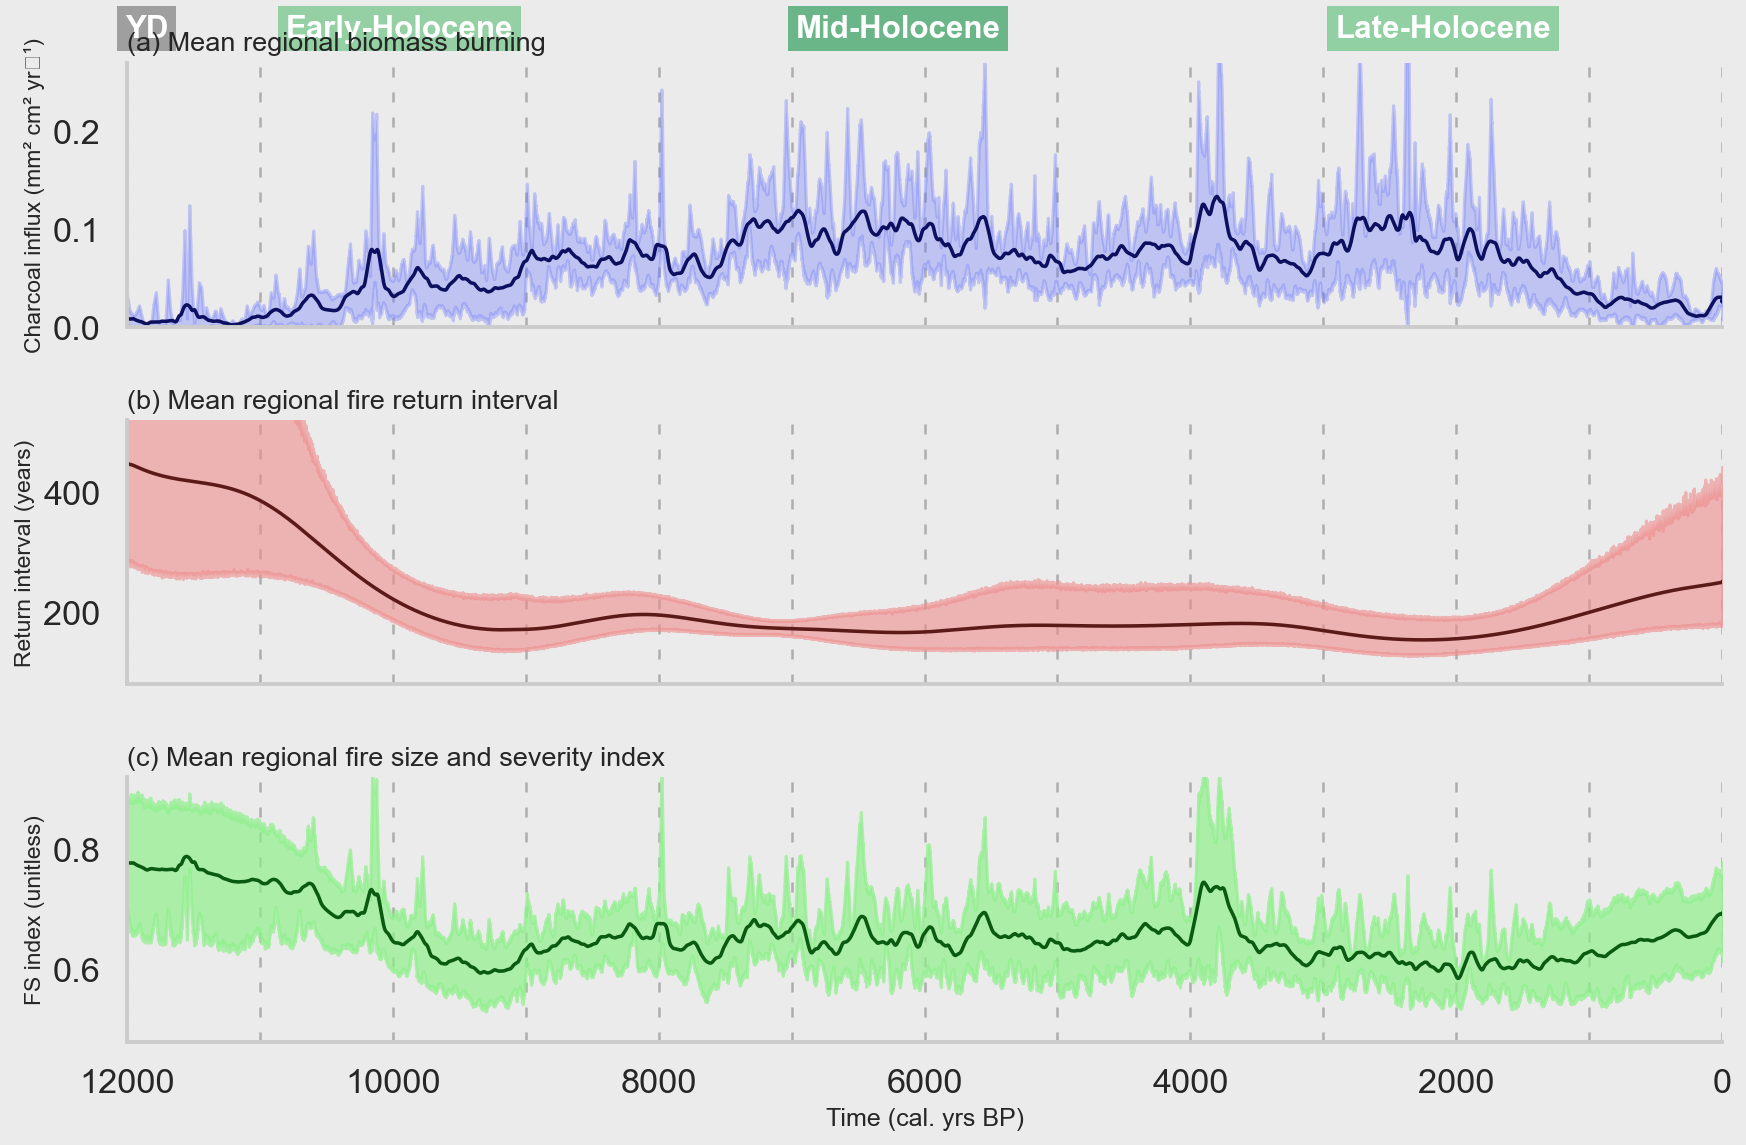
\includegraphics[width=0.95\textwidth]{figures_feu/fig_02_regional_fire_history.png}
\caption{Historique r\'egional du feu: (a) biomasse br\^ul\'ee r\'egionale, (b) intervalle de retour du feu, (c) indice de taille / s\'ev\'erit\'e.}
\label{fig:regional_history}
\end{figure}

\subsection*{Lecture synth\'etique}
Le signal r\'egional sugg\`ere trois phases principales:
\begin{itemize}
\item un d\'ebut de s\'erie plus ancien avec des feux relativement espac\'es mais un indice de taille / s\'ev\'erit\'e \'elev\'e;
\item un coeur holoc\`ene marqu\'e par des intervalles de retour plus courts et une biomasse br\^ul\'ee plus forte;
\item une tendance r\'ecente \`a la baisse de la biomasse br\^ul\'ee, avec une remont\'ee mod\'er\'ee de l'intervalle de retour.
\end{itemize}

Ces motifs sont coh\'erents avec les interpr\'etations d\'etaill\'ees dans le notebook d'exploration~\cite{nb_explo}.

\section{Donn\'ees par lac}
Les figures suivantes documentent la variabilit\'e inter-lacs. Elles montrent que le signal n'est pas homog\`ene: certains sites dominent des p\'eriodes de forte activit\'e, alors que d'autres contribuent plus faiblement et de mani\`ere plus intermittente.

\begin{figure}[H]
\centering
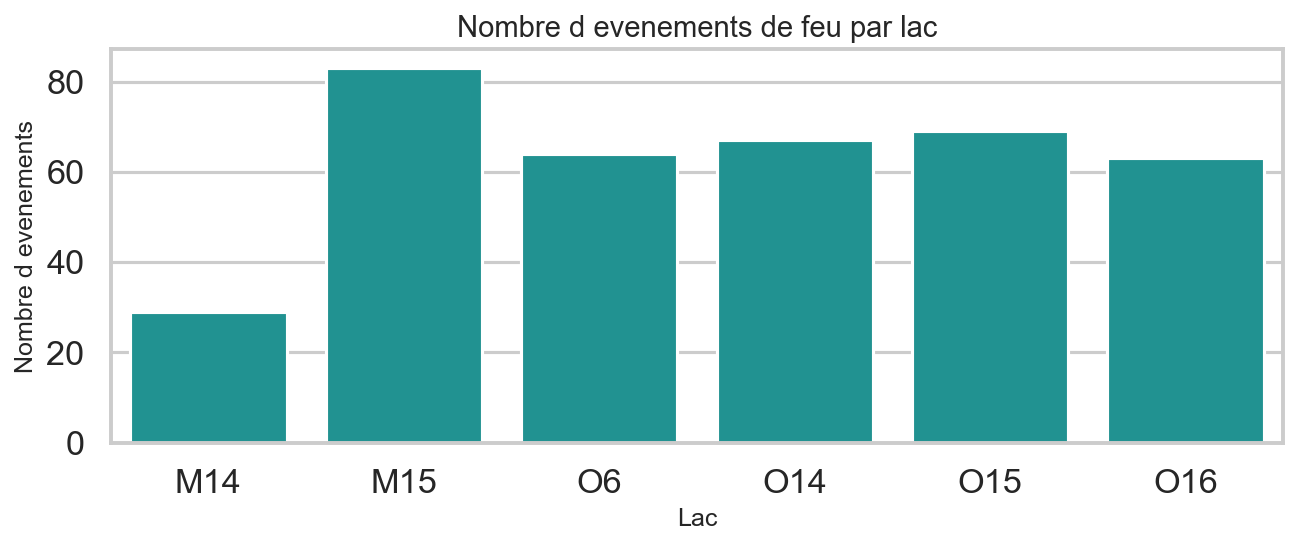
\includegraphics[width=0.8\textwidth]{figures_feu/fig_02_evenements_par_lac.png}
\caption{Nombre total d'\'ev\'enements de feu par lac.}
\label{fig:count_lakes}
\end{figure}

\begin{figure}[H]
\centering
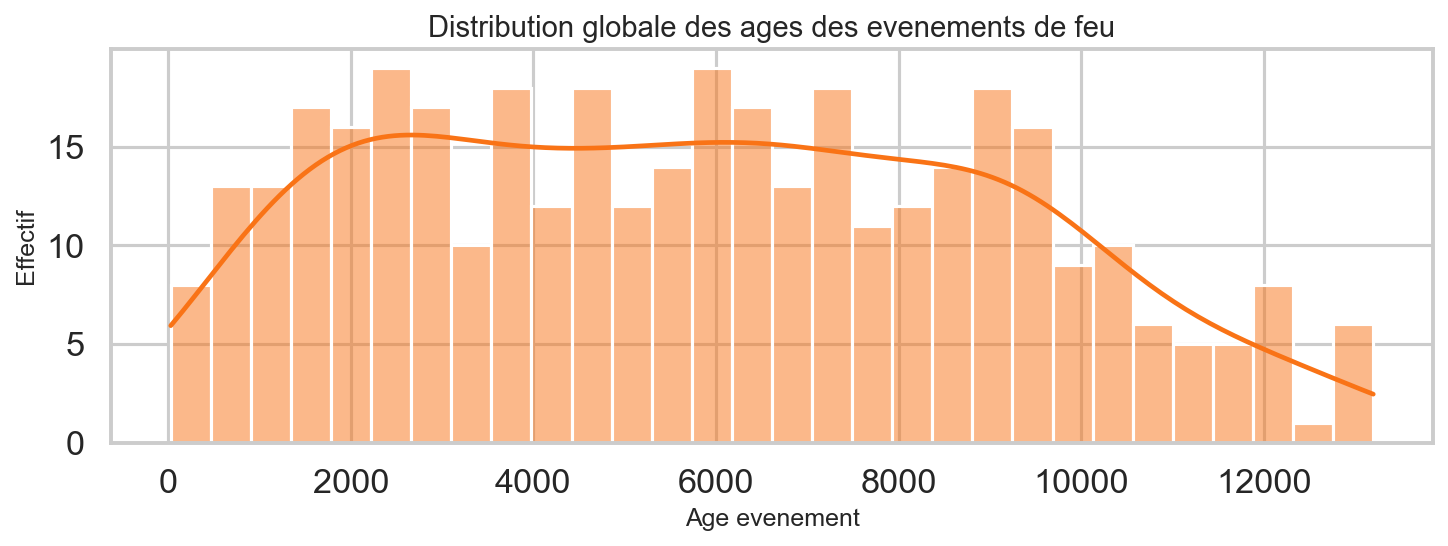
\includegraphics[width=0.85\textwidth]{figures_feu/fig_03_distribution_ages_evenements.png}
\caption{Distribution globale des \^ages des occurrences de feu.}
\label{fig:age_distribution}
\end{figure}

\begin{figure}[H]
\centering
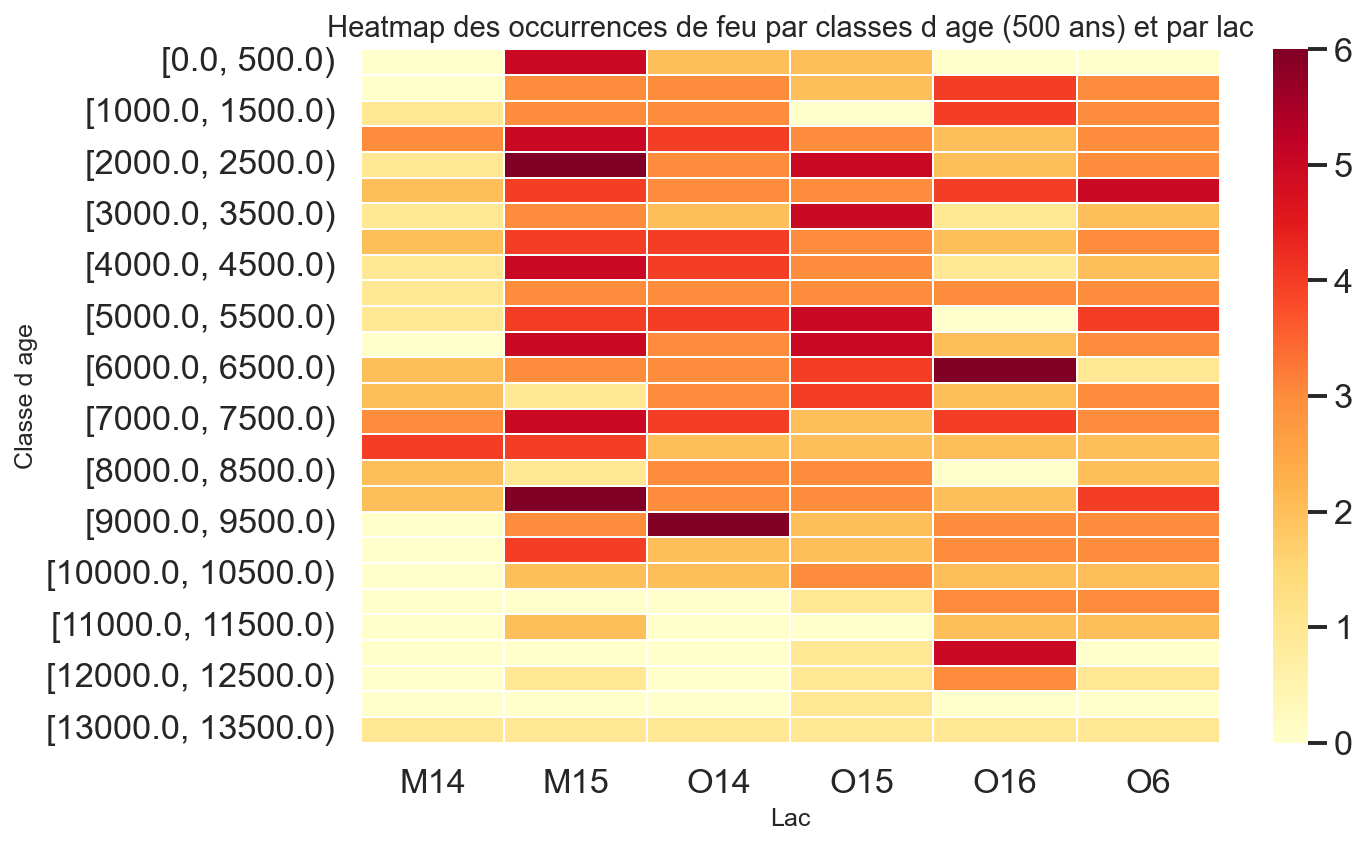
\includegraphics[width=0.95\textwidth]{figures_feu/fig_04_heatmap_occurrences_par_lac_500ans.png}
\caption{Heatmap des occurrences de feu par classes de 500 ans et par lac.}
\label{fig:heatmap_500}
\end{figure}

\begin{figure}[H]
\centering
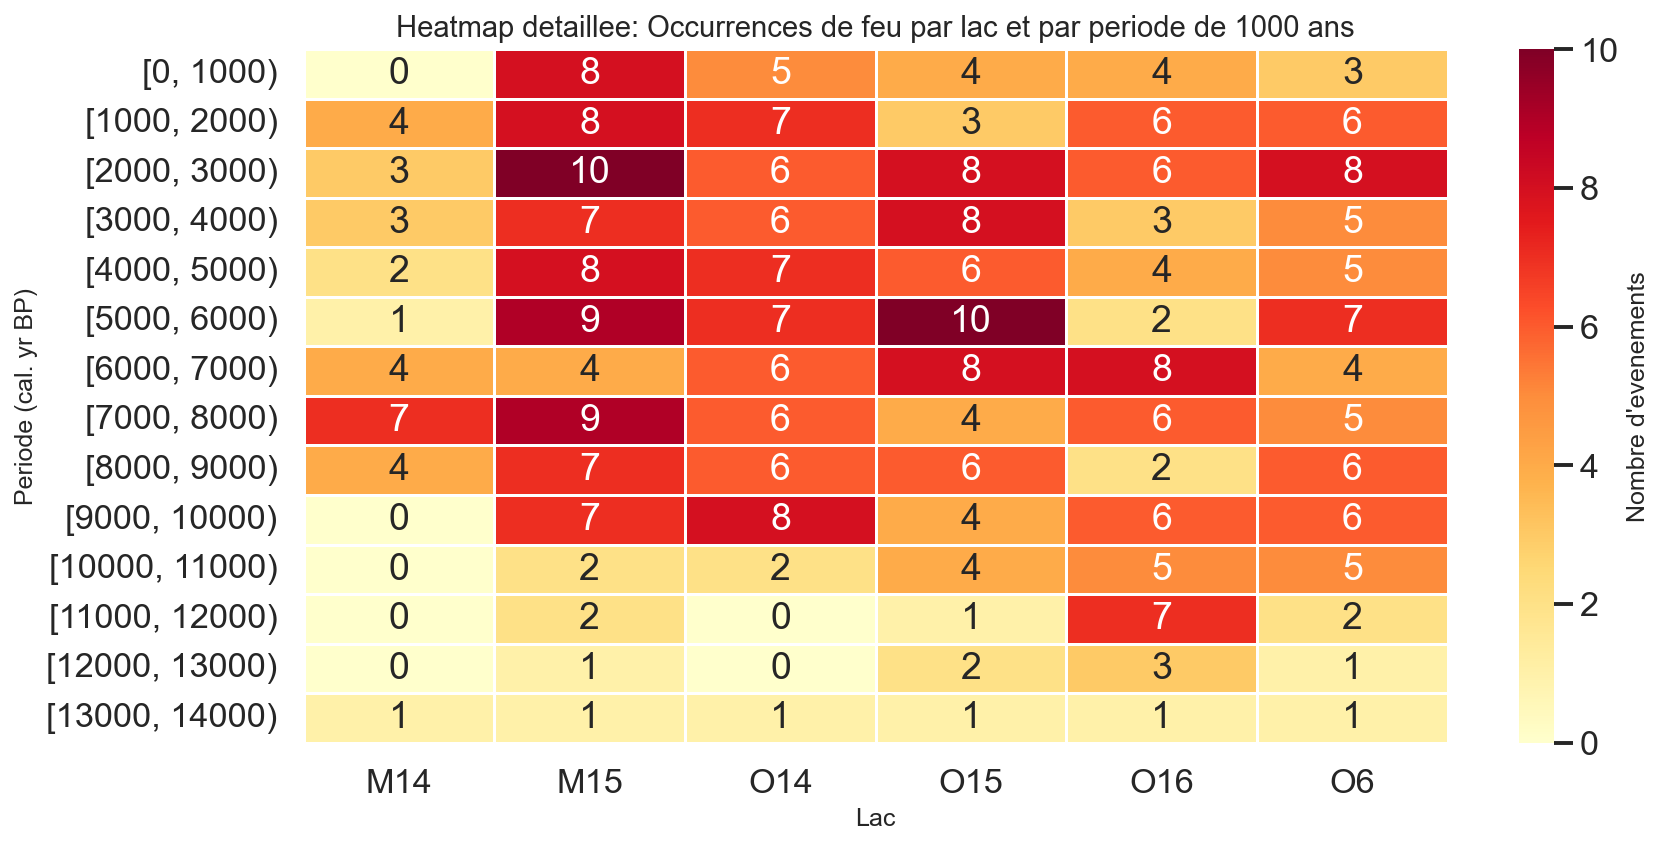
\includegraphics[width=0.95\textwidth]{figures_feu/fig_05_heatmap_occurrences_par_lac_1000ans.png}
\caption{Heatmap des occurrences de feu par classes de 1\,000 ans et par lac.}
\label{fig:heatmap_1000}
\end{figure}

\begin{figure}[H]
\centering
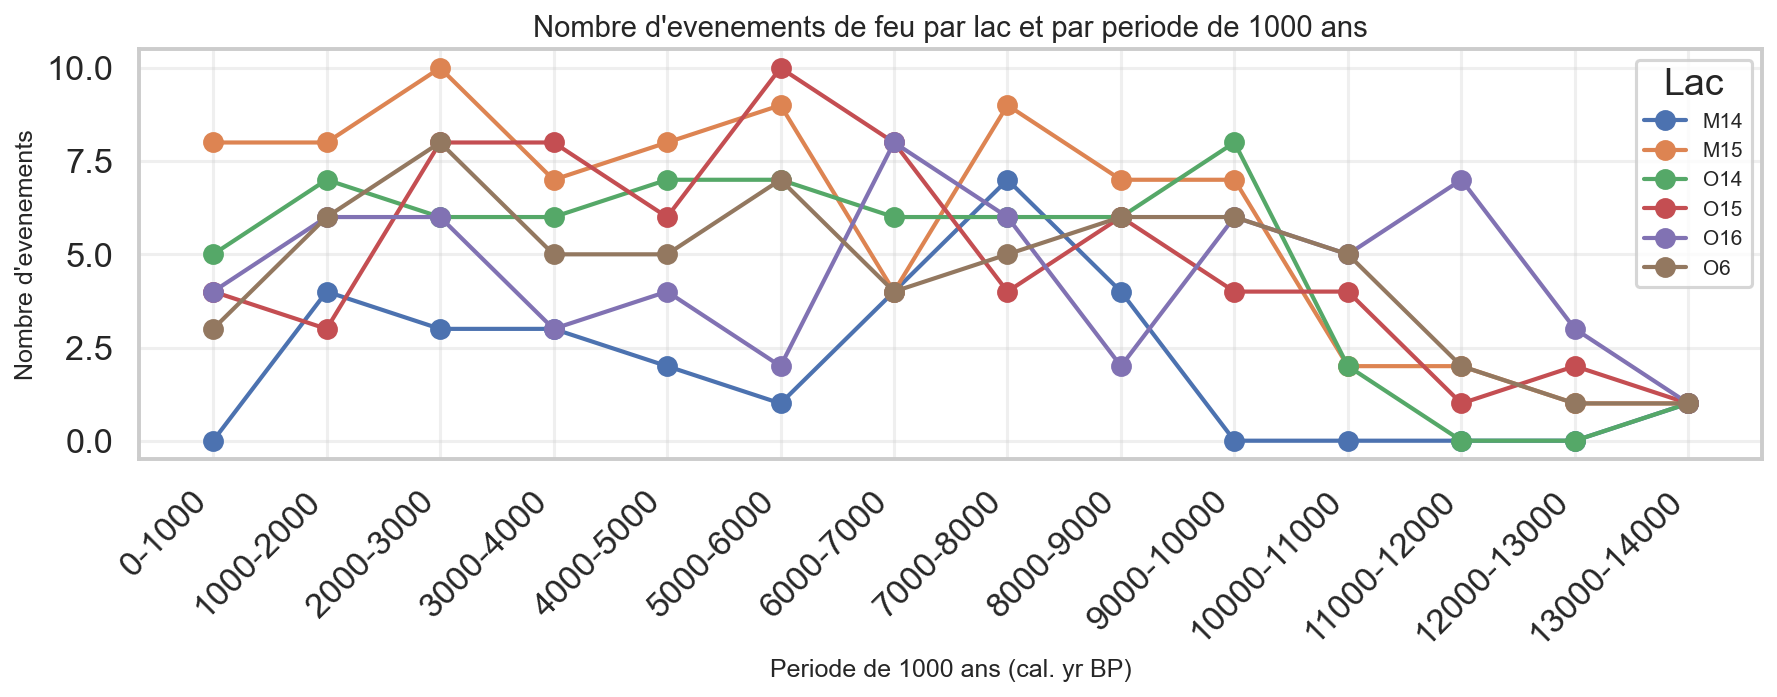
\includegraphics[width=0.95\textwidth]{figures_feu/fig_06_timeline_occurrences_par_lac_1000ans.png}
\caption{S\'erie temporelle du nombre d'\'ev\'enements par lac, agr\'eg\'ee par tranches de 1\,000 ans.}
\label{fig:timeline_1000}
\end{figure}

\subsection*{Lecture des figures par lac}
Les graphiques mettent en \'evidence une hi\'erarchie claire:
\begin{itemize}
\item \textbf{M15} est le site le plus actif, avec 83 occurrences et plusieurs pics marqu\'es au milieu de l'Holoc\`ene.
\item \textbf{O15}, \textbf{O14} et \textbf{O16} jouent un r\^ole interm\'ediaire, avec des contributions r\'eparties sur plusieurs mill\'enaires.
\item \textbf{M14} contribue le moins au signal global et pr\'esente plusieurs intervalles de faible activit\'e.
\end{itemize}

La densit\'e maximale des occurrences se situe globalement entre 2\,000 et 9\,000 ans avant le pr\'esent, tandis que les extr\^emes de la chronologie sont plus pauvres en \'ev\'enements.

\section{Chronologies locales repr\'esentatives}
Les chronologies ci-dessous sont utiles pour lire les diff\'erences locales entre sites et comprendre quels lacs dominent certains segments temporels.

\begin{figure}[H]
\centering
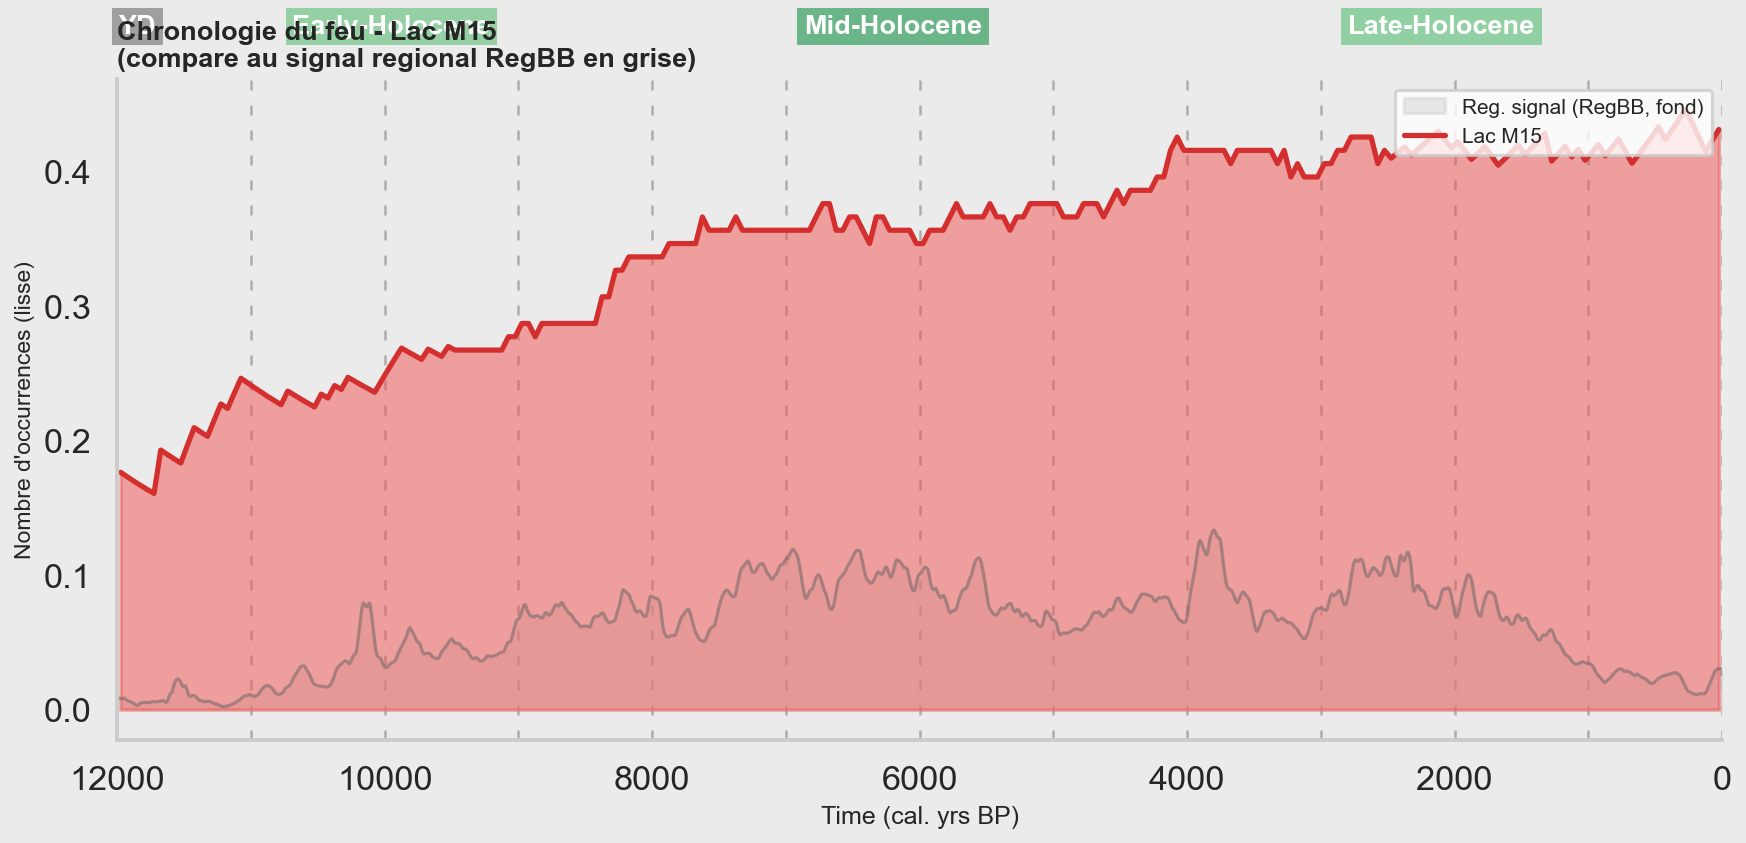
\includegraphics[width=0.95\textwidth]{figures_feu/fig_lac_M15_chronologie.png}
\caption{Chronologie locale du lac M15 compar\'ee au signal r\'egional.}
\end{figure}

\begin{figure}[H]
\centering
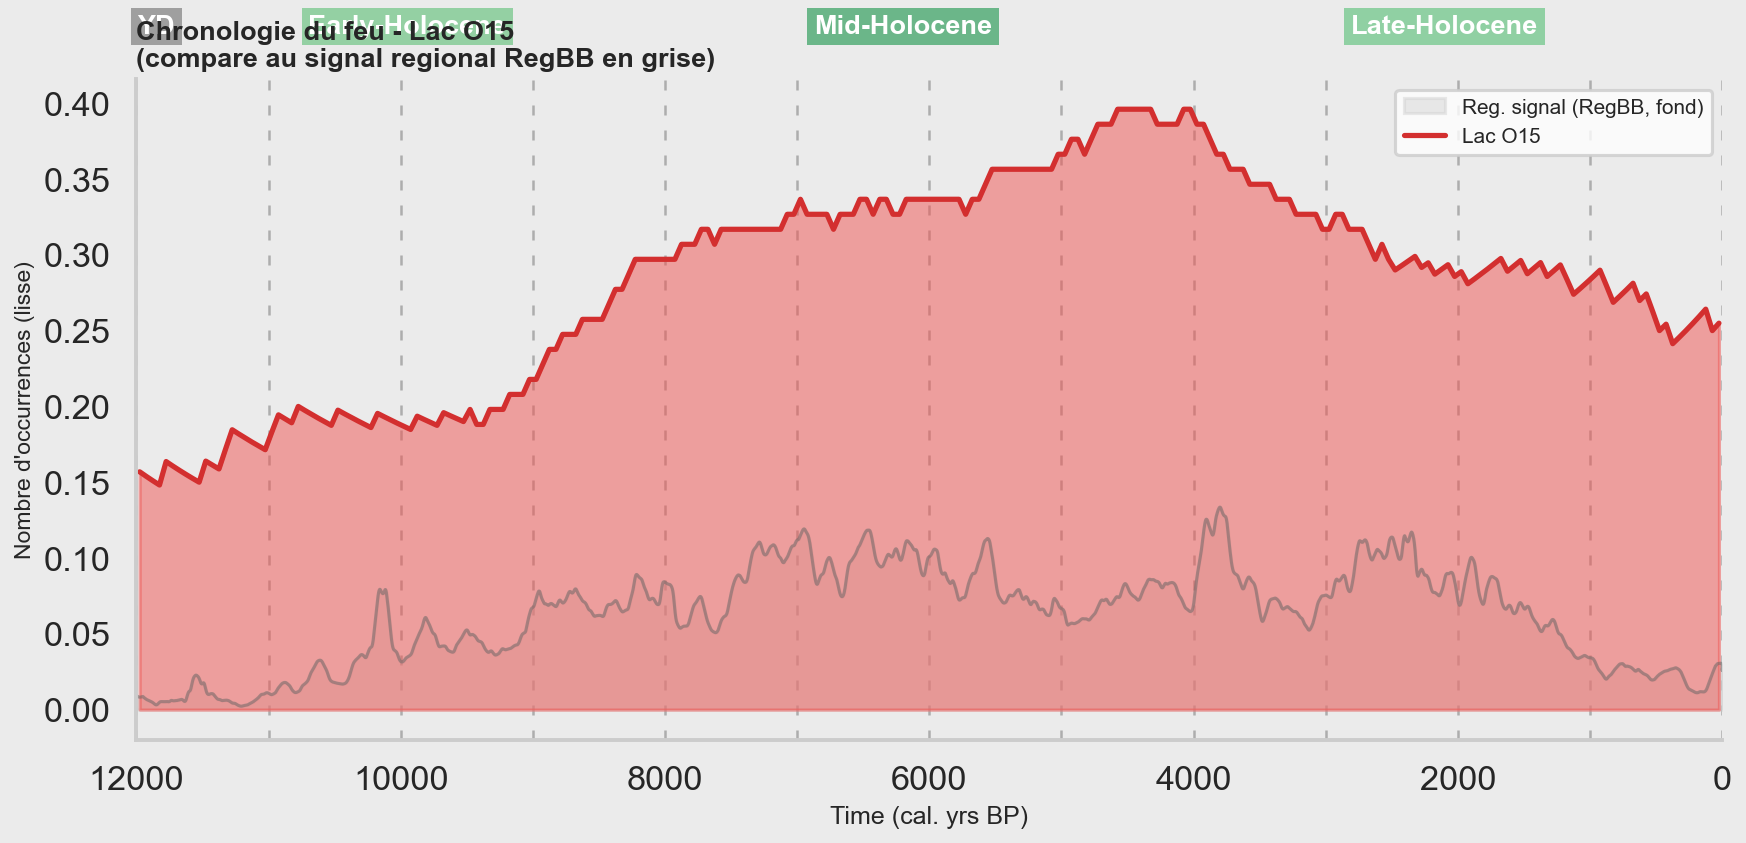
\includegraphics[width=0.95\textwidth]{figures_feu/fig_lac_O15_chronologie.png}
\caption{Chronologie locale du lac O15 compar\'ee au signal r\'egional.}
\end{figure}

\begin{figure}[H]
\centering
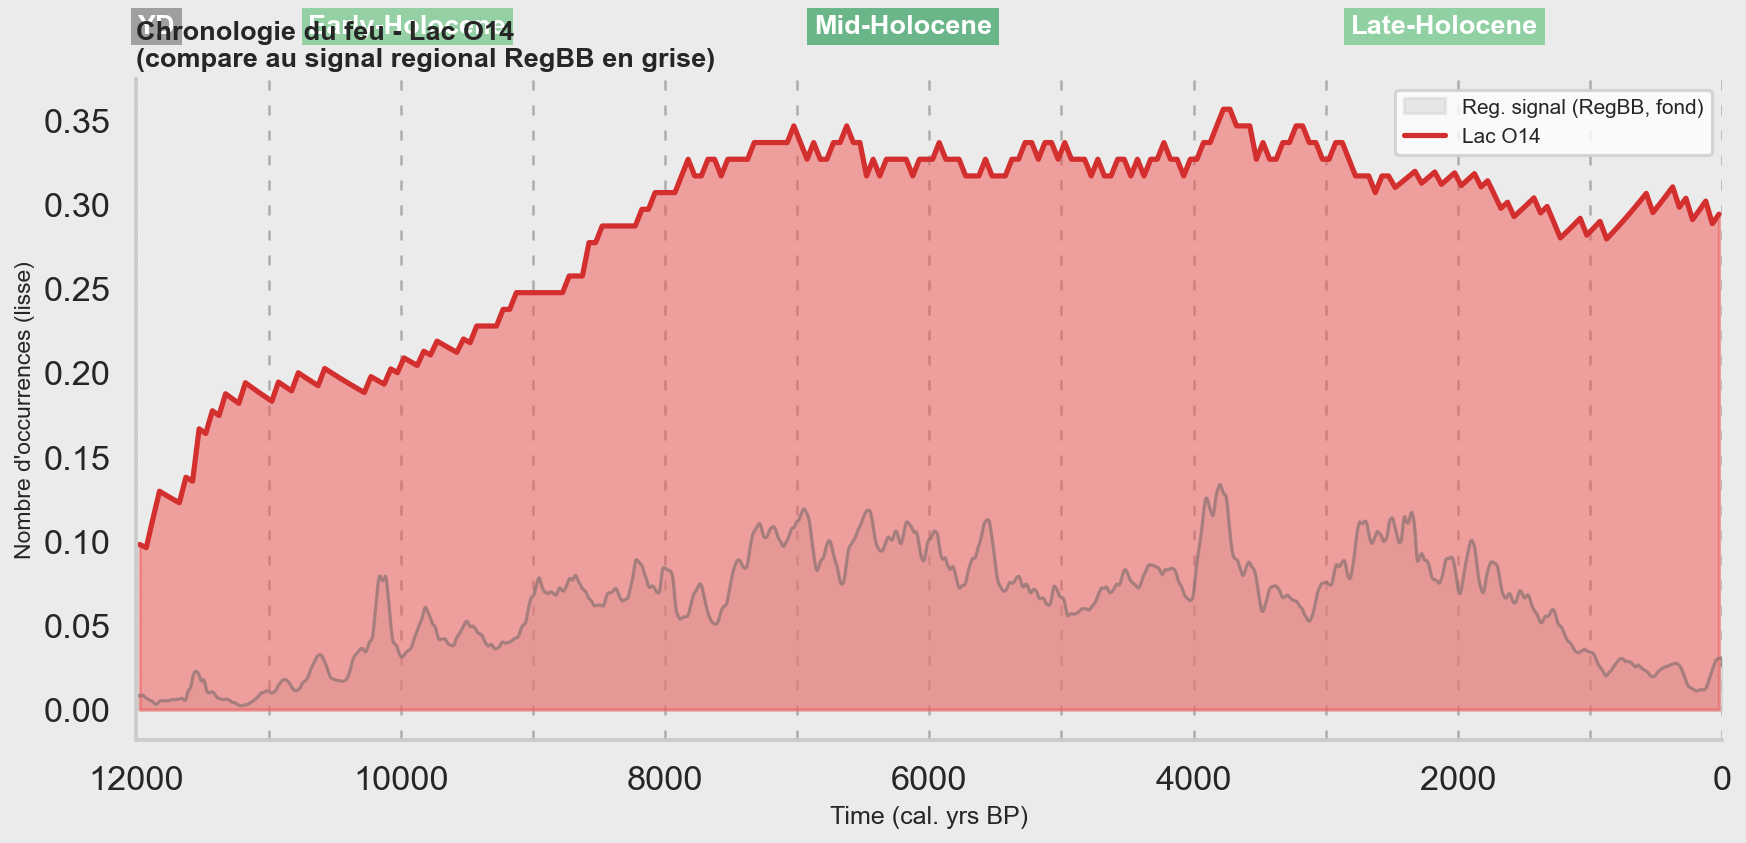
\includegraphics[width=0.95\textwidth]{figures_feu/fig_lac_O14_chronologie.png}
\caption{Chronologie locale du lac O14 compar\'ee au signal r\'egional.}
\end{figure}

\begin{figure}[H]
\centering
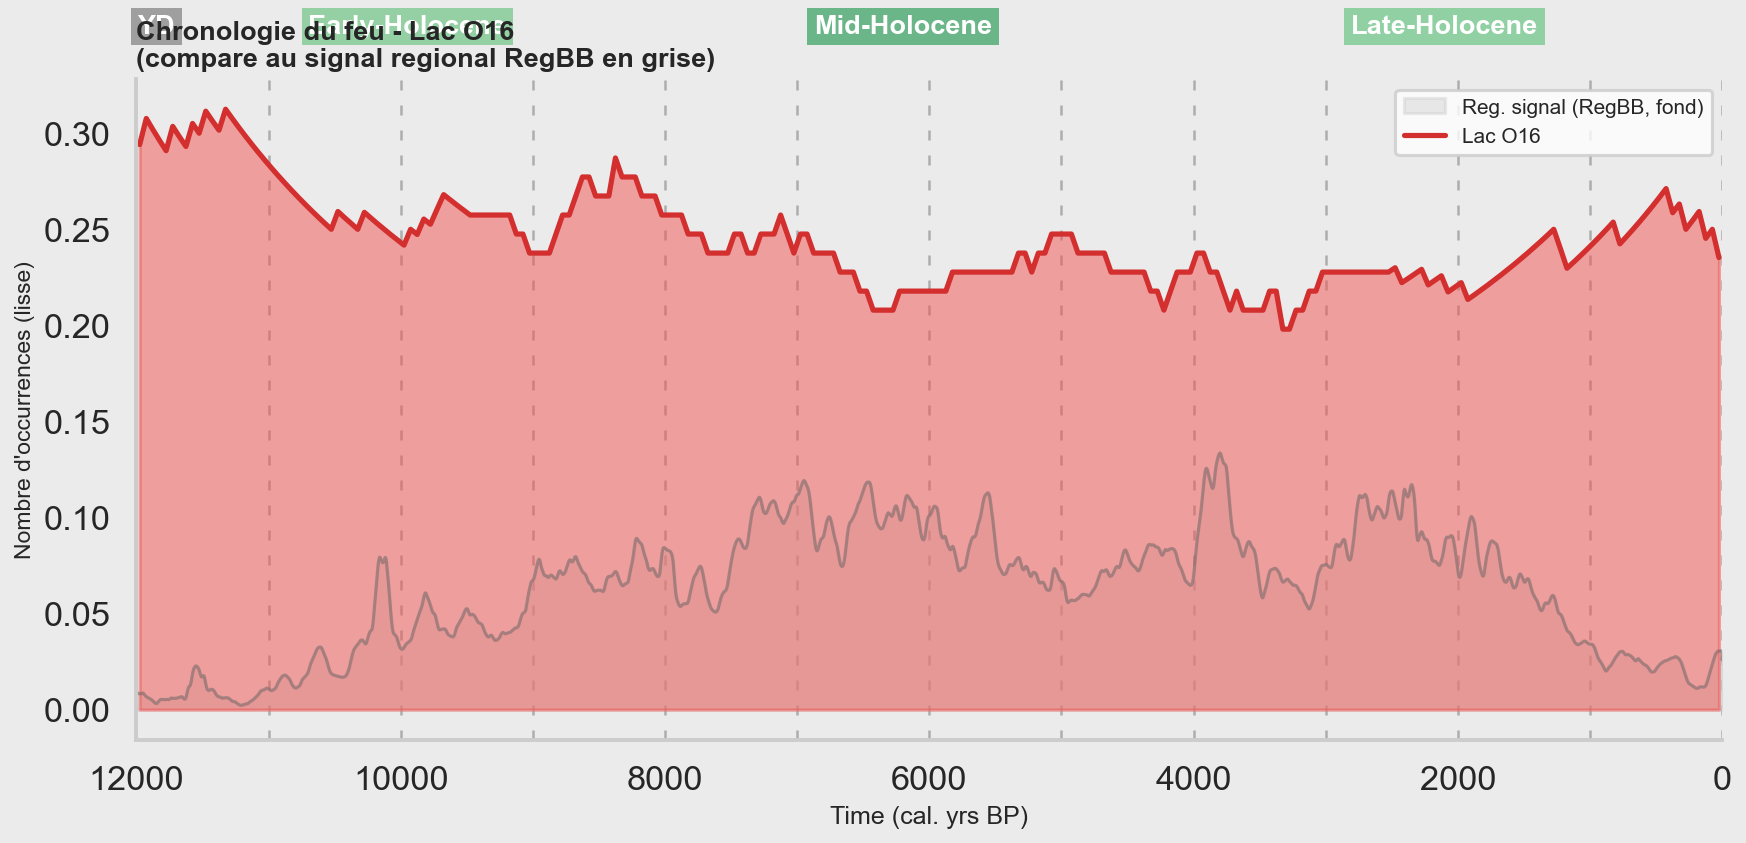
\includegraphics[width=0.95\textwidth]{figures_feu/fig_lac_O16_chronologie.png}
\caption{Chronologie locale du lac O16 compar\'ee au signal r\'egional.}
\end{figure}

\begin{figure}[H]
\centering
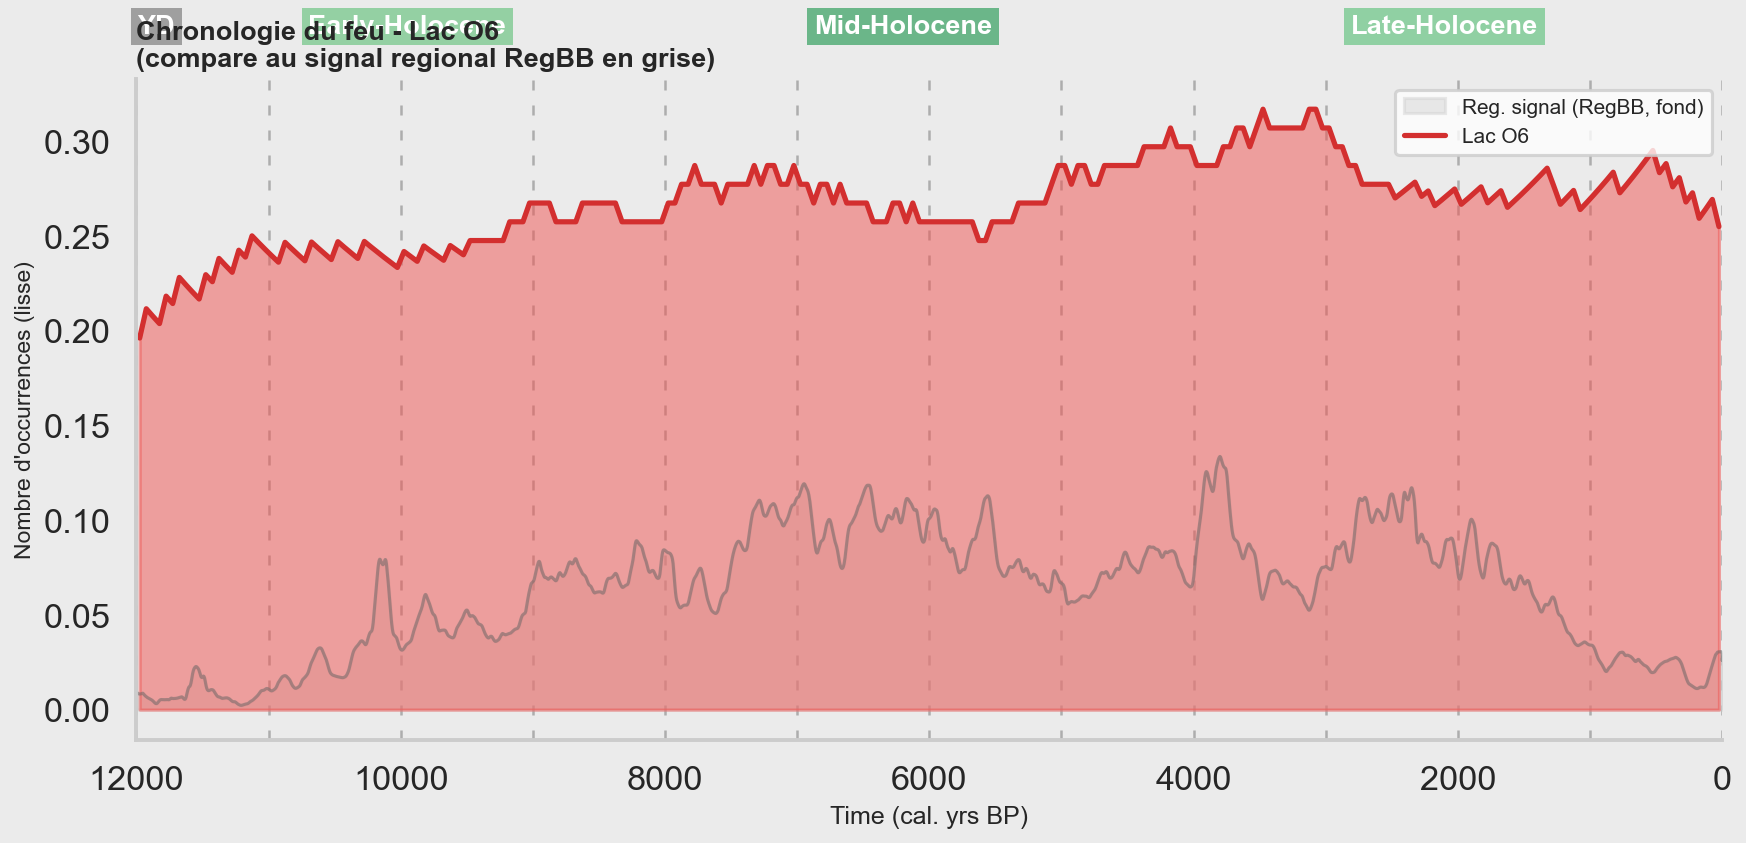
\includegraphics[width=0.95\textwidth]{figures_feu/fig_lac_O6_chronologie.png}
\caption{Chronologie locale du lac O6 compar\'ee au signal r\'egional.}
\end{figure}

\begin{figure}[H]
\centering
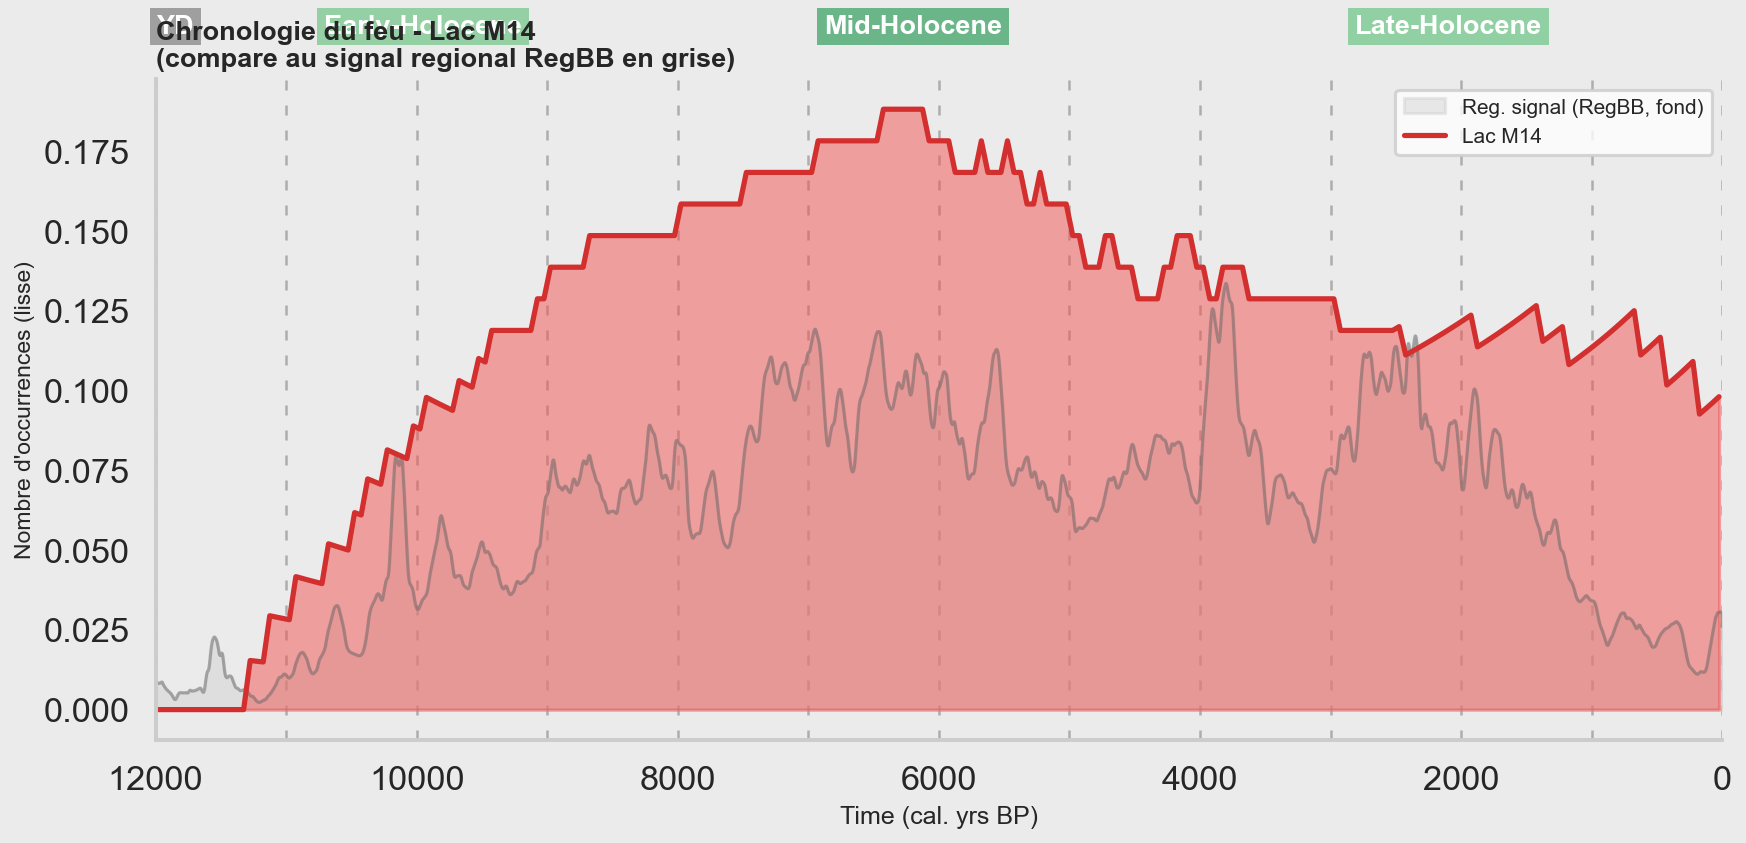
\includegraphics[width=0.95\textwidth]{figures_feu/fig_lac_M14_chronologie.png}
\caption{Chronologie locale du lac M14 compar\'ee au signal r\'egional.}
\end{figure}

\section{Zoom temporels utiles}
Les figures de zoom permettent de d\'ecouper la chronologie en fen\^etres de 2\,000 ans et de suivre la dynamique locale sans perdre le contexte r\'egional.

\begin{figure}[H]
\centering
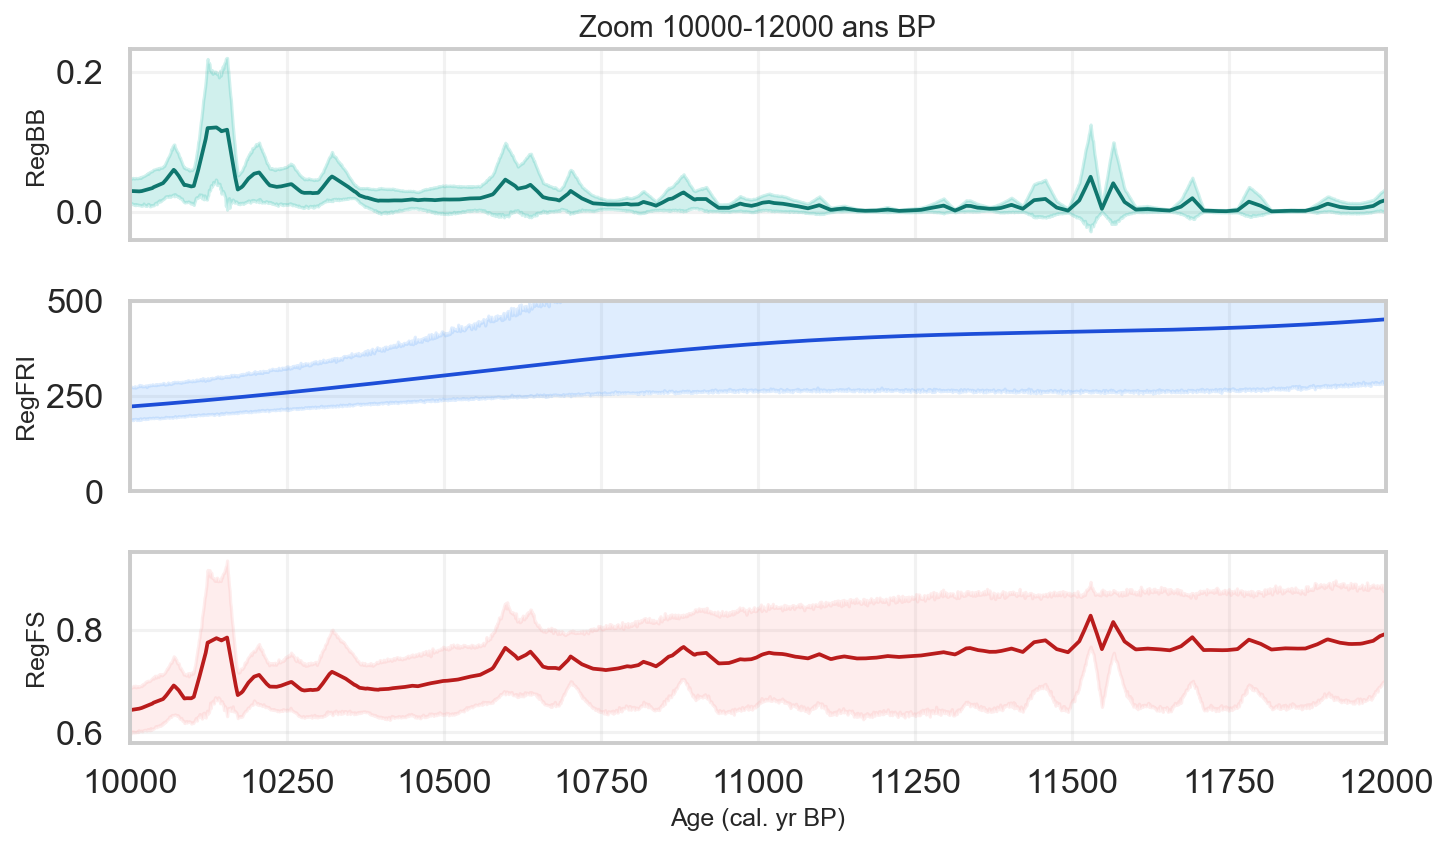
\includegraphics[width=0.95\textwidth]{figures_feu/fig_05_zoom_10000_12000_bp.png}
\caption{Zoom 10\,000--12\,000 ans BP.}
\end{figure}

\begin{figure}[H]
\centering
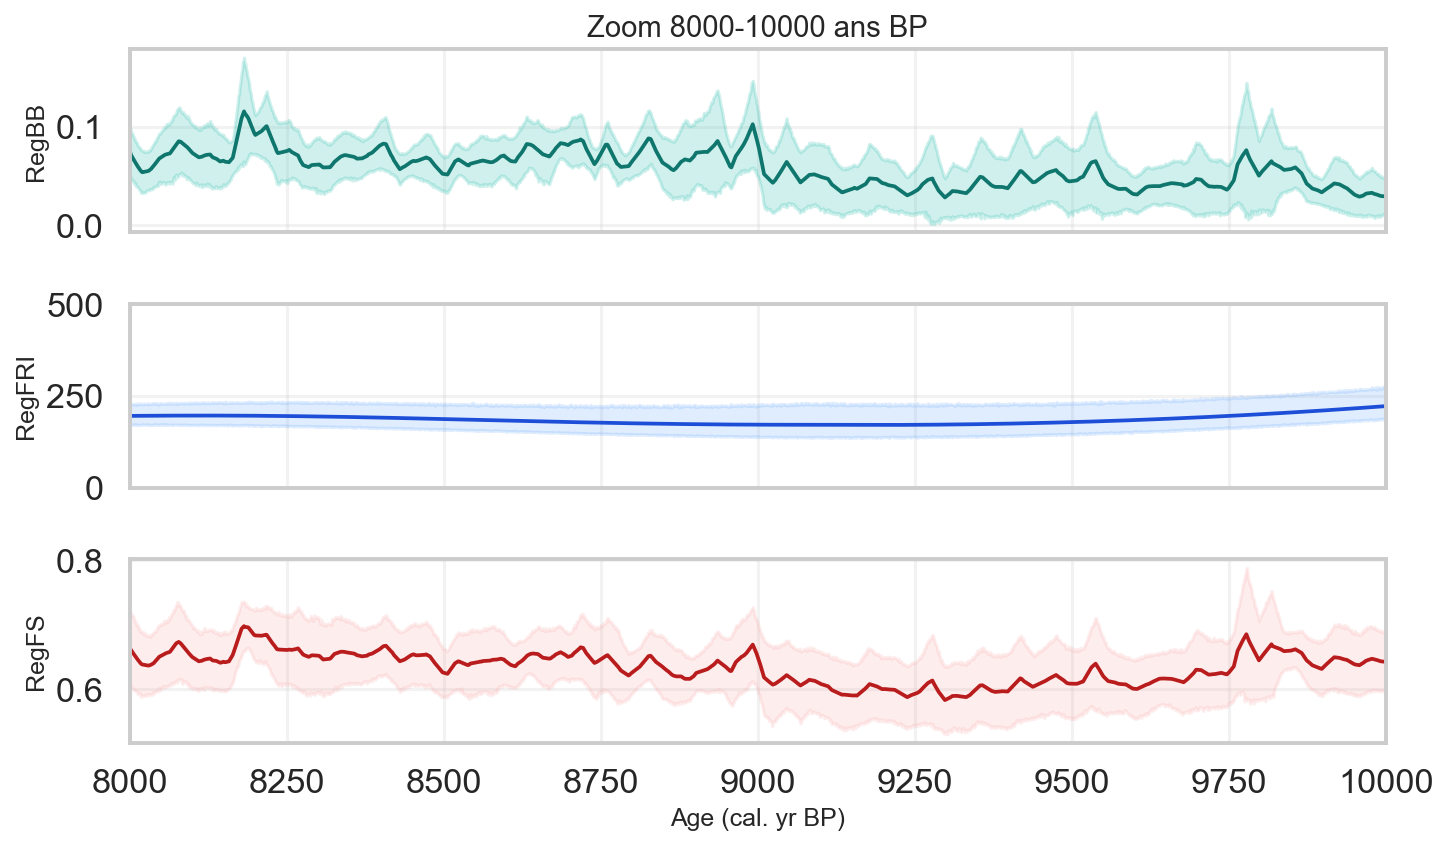
\includegraphics[width=0.95\textwidth]{figures_feu/fig_05_zoom_8000_10000_bp.png}
\caption{Zoom 8\,000--10\,000 ans BP.}
\end{figure}

\begin{figure}[H]
\centering
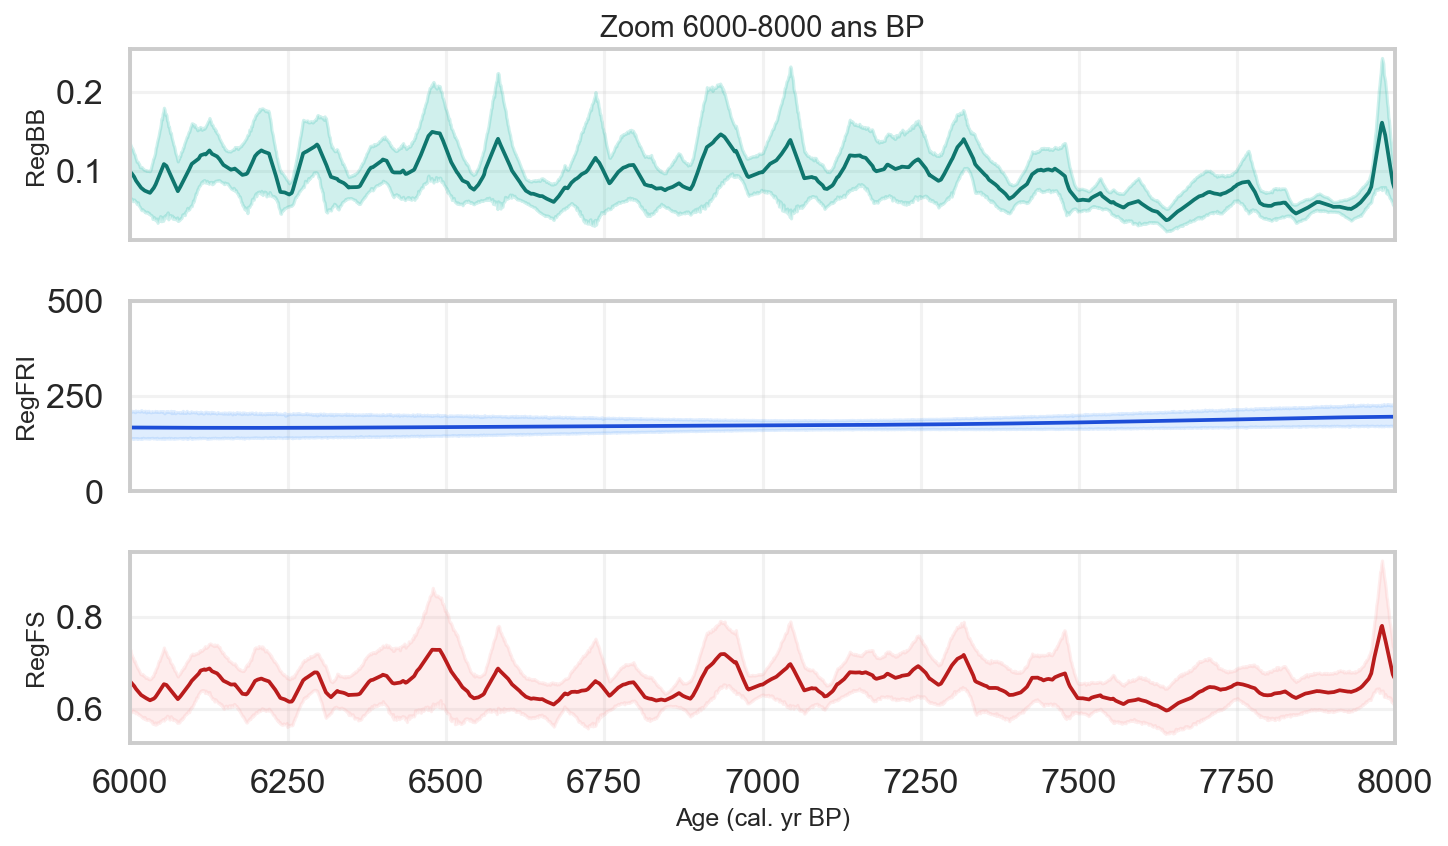
\includegraphics[width=0.95\textwidth]{figures_feu/fig_05_zoom_6000_8000_bp.png}
\caption{Zoom 6\,000--8\,000 ans BP.}
\end{figure}

\begin{figure}[H]
\centering
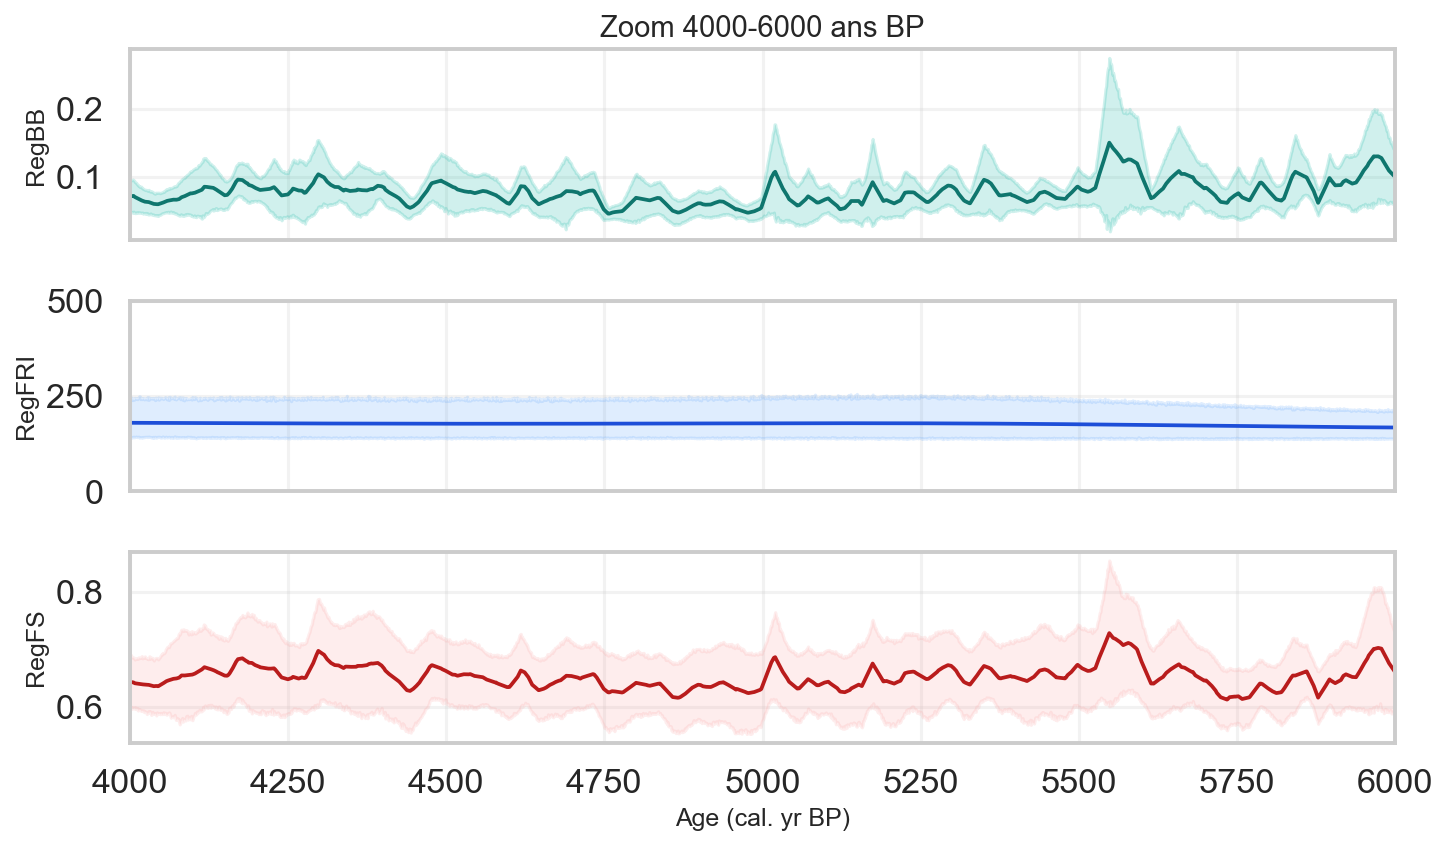
\includegraphics[width=0.95\textwidth]{figures_feu/fig_05_zoom_4000_6000_bp.png}
\caption{Zoom 4\,000--6\,000 ans BP.}
\end{figure}

\begin{figure}[H]
\centering
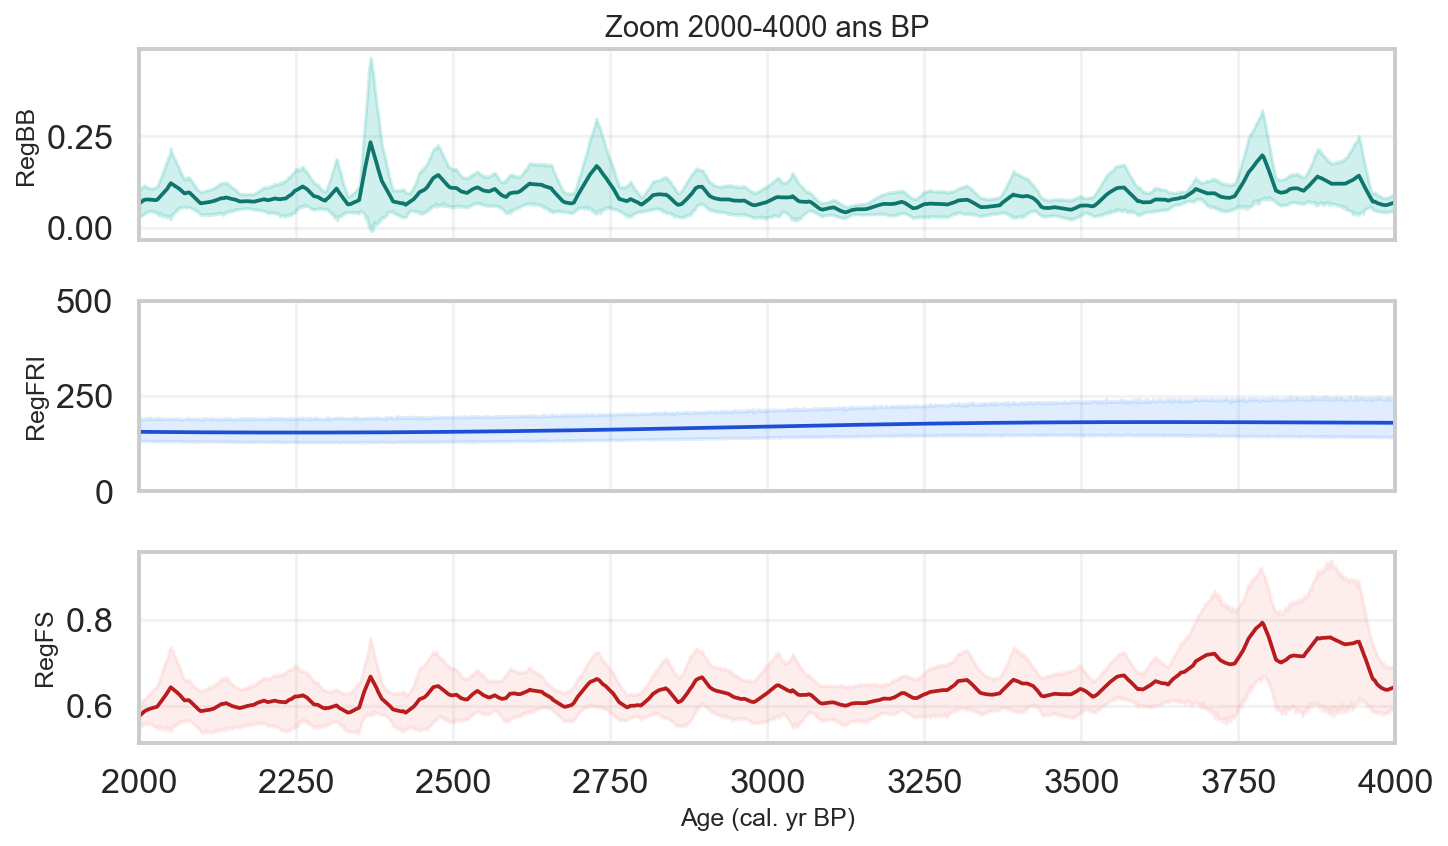
\includegraphics[width=0.95\textwidth]{figures_feu/fig_05_zoom_2000_4000_bp.png}
\caption{Zoom 2\,000--4\,000 ans BP.}
\end{figure}

\begin{figure}[H]
\centering
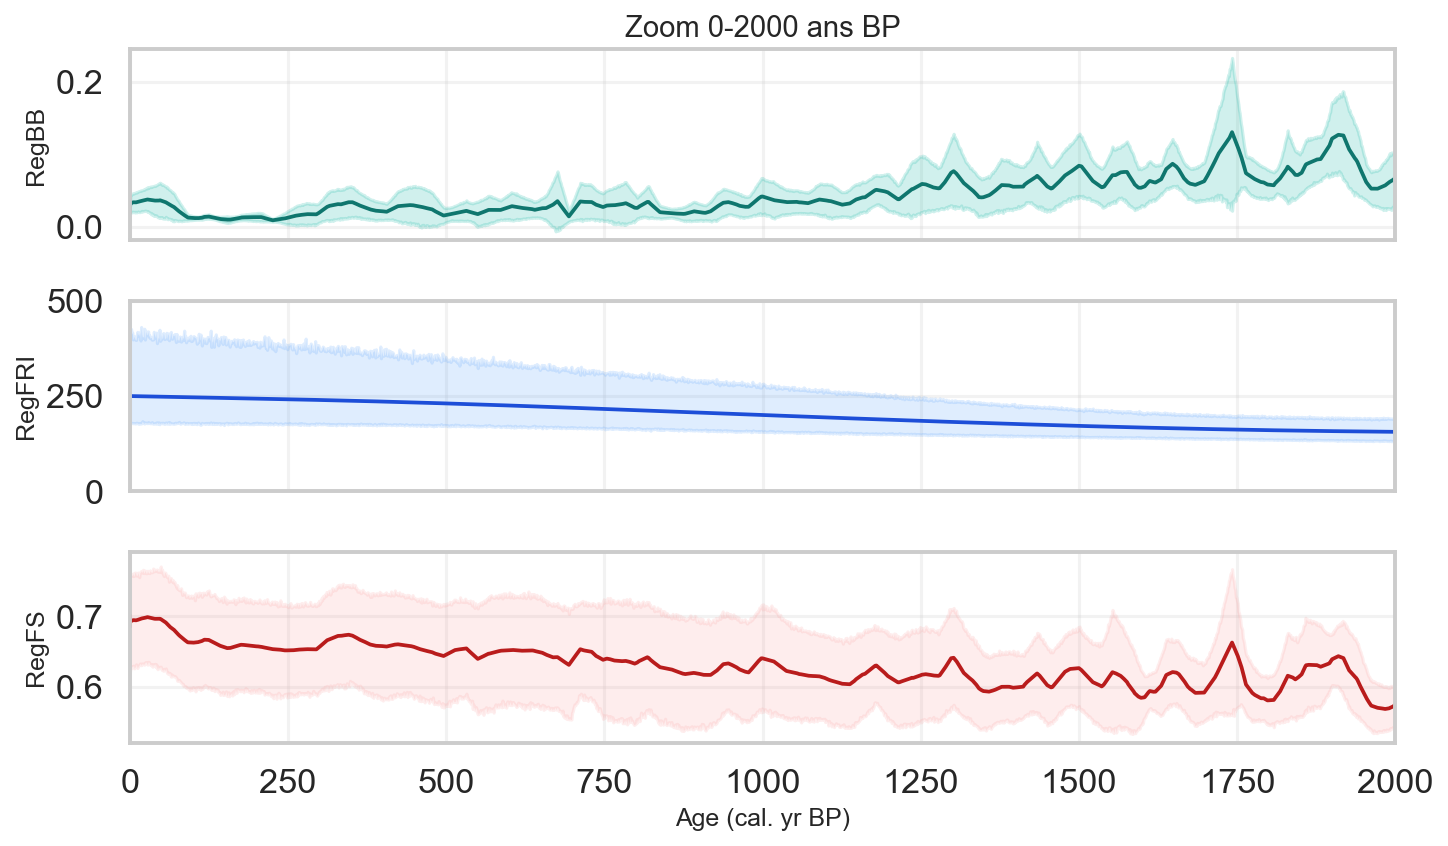
\includegraphics[width=0.95\textwidth]{figures_feu/fig_05_zoom_0_2000_bp.png}
\caption{Zoom 0--2\,000 ans BP.}
\end{figure}

\begin{figure}[H]
\centering
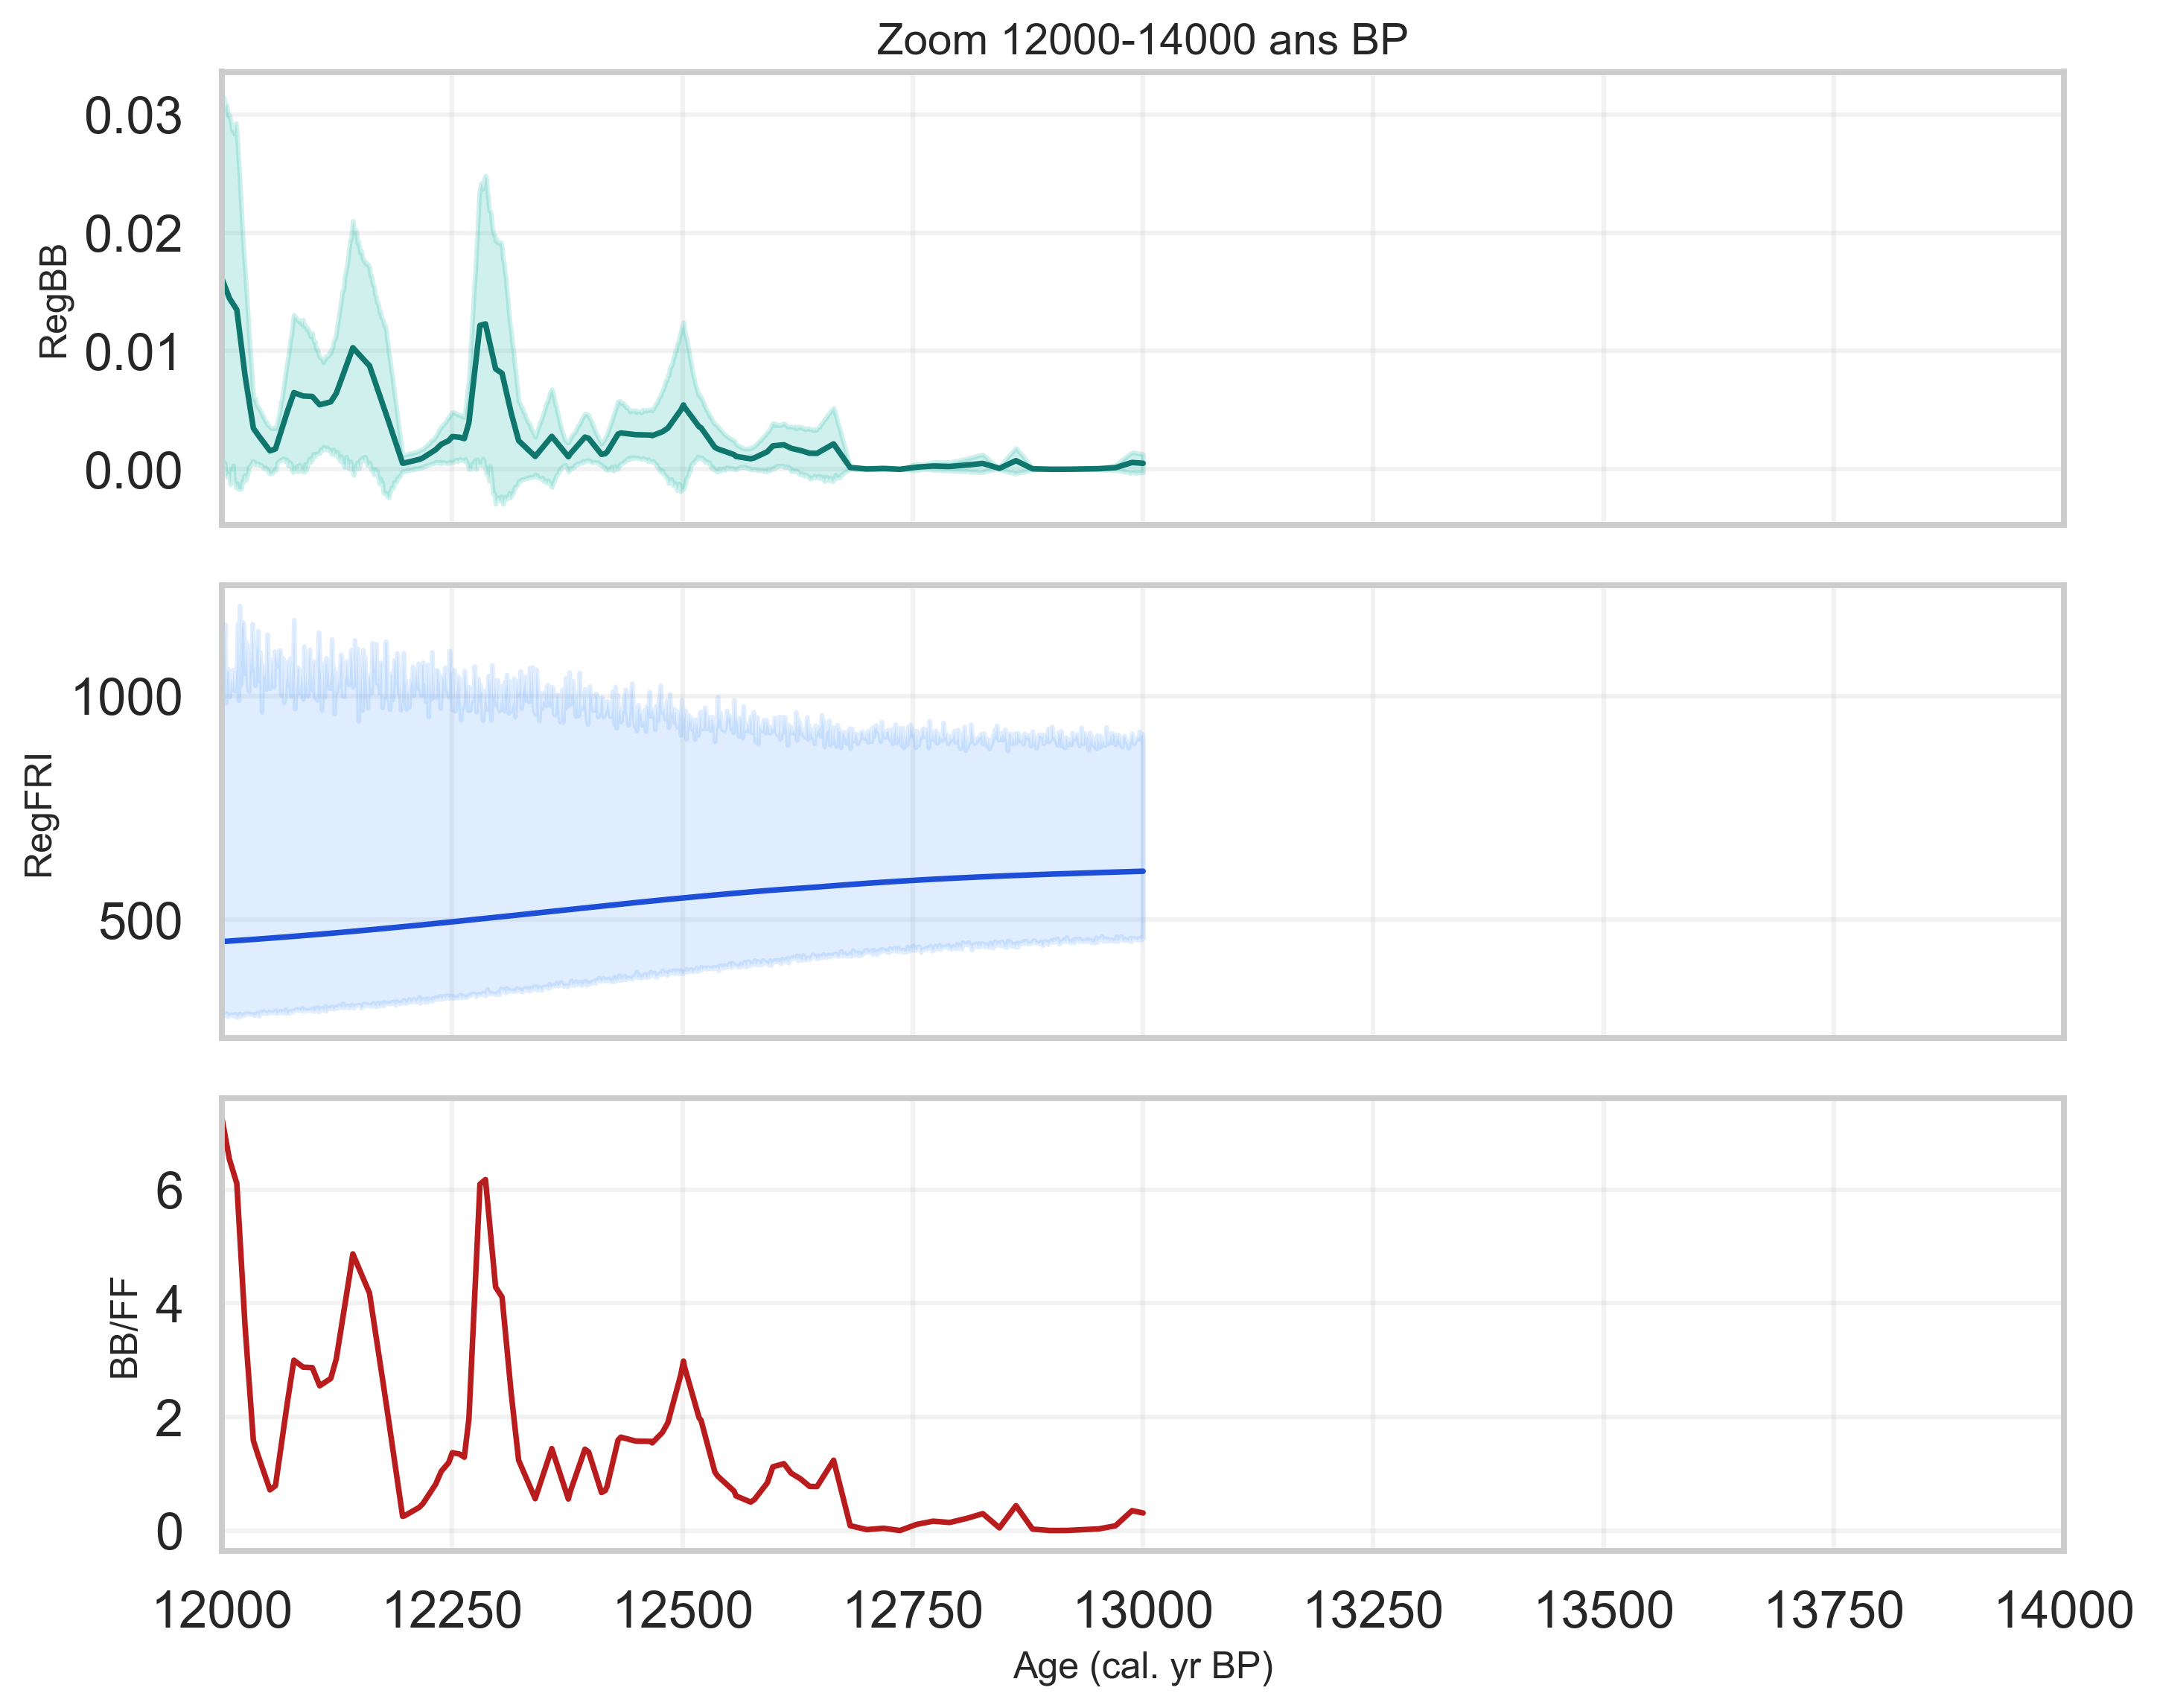
\includegraphics[width=0.95\textwidth]{figures_feu/fig_05_zoom_12000_14000_bp.png}
\caption{Zoom 12\,000--14\,000 ans BP.}
\end{figure}

\section{Conclusion}
Les donn\'ees montrent un signal r\'egional du feu clairement structur\'e dans le temps, avec un maximum d'activit\'e au centre de l'Holoc\`ene et une forte h\'et\'erog\'en\'eit\'e entre lacs. Les fichiers \texttt{FFBootCISap.csv}, \texttt{BBBootCISap.csv} et \texttt{FSBootCISap.csv} constituent la base des proxys r\'egionaux, tandis que \texttt{Lake\_fire\_frequency\_24nov2023.csv} permet de lire la distribution spatiale et temporelle des occurrences.

Le notebook d'exploration~\cite{nb_explo} reste la r\'ef\'erence principale pour le d\'etail des traitements et des figures; le document technique sur les mod\`eles~\cite{doc_modeles} peut \^etre r\'eutilis\'e ensuite pour relier cette description des donn\'ees aux pr\'evisions s\'equentielles.

\begin{thebibliography}{9}
\bibitem{nb_explo}
\texttt{Analyse\_exploratoire\_donnees.ipynb}, notebook d'exploration des donn\'ees dans le workspace \textit{Foret\_Boreal}.

\bibitem{doc_modeles}
\texttt{document\_architecture\_modeles\_seq.tex}, document technique sur l'architecture des mod\`eles s\'equentiels.

\bibitem{pres_feu}
\texttt{presentation\_feu\_boreal\_beamer.tex}, synth\`ese de pr\'esentation du projet.
\end{thebibliography}

\end{document}